% !TEX root = ../report.tex

\chapter{Evaluation}

\minitoc

This chapter will be used to evaluate the work and the results drawn from the research done. This chapter will also discuss why the outcome ended up as it did. This includes obstacles met during research, design and implementation, how issues could have been handled in a different way and significants of the findings.

\clearpage


\section{Development Process}
The development process used in the project was not modeled after any particular rigid paradigm of development, but instead followed the natural workflow of the individual programmers. Even though a particular type of predetermined workflow was not applied, there were clear tendencies in how the development happened.

The team started out with less rigid requirements. In the beginning of the project, they were something along the lines of: Store the Netflix movies in an accessible database, retrieve tweets about movies from Twitter and store them in the same database.

Each of these requirements were attacked by gathering ruby gems that seemed like they would be suitable for fulfilling the requirement. A proof of concept implementing the requirement was then created in an environment separate from other parts of the project.

As time progressed and more requirements were fulfilled the implementations of the requirements were fused into a larger project. As the project increased in complexity, and the requirements were fulfilled, more requirements emerged. They were implemented and added to the larger code base.

At one point, the code base was beginning to get complex and fusing implementations of requirements into this code base was getting difficult. This implied the need of an architecture. A basic architecture was created and the code was refactored. This process continued looping. An illustration can be seen in figure~\ref{figure:development-cycle}

\begin{figure}[H]
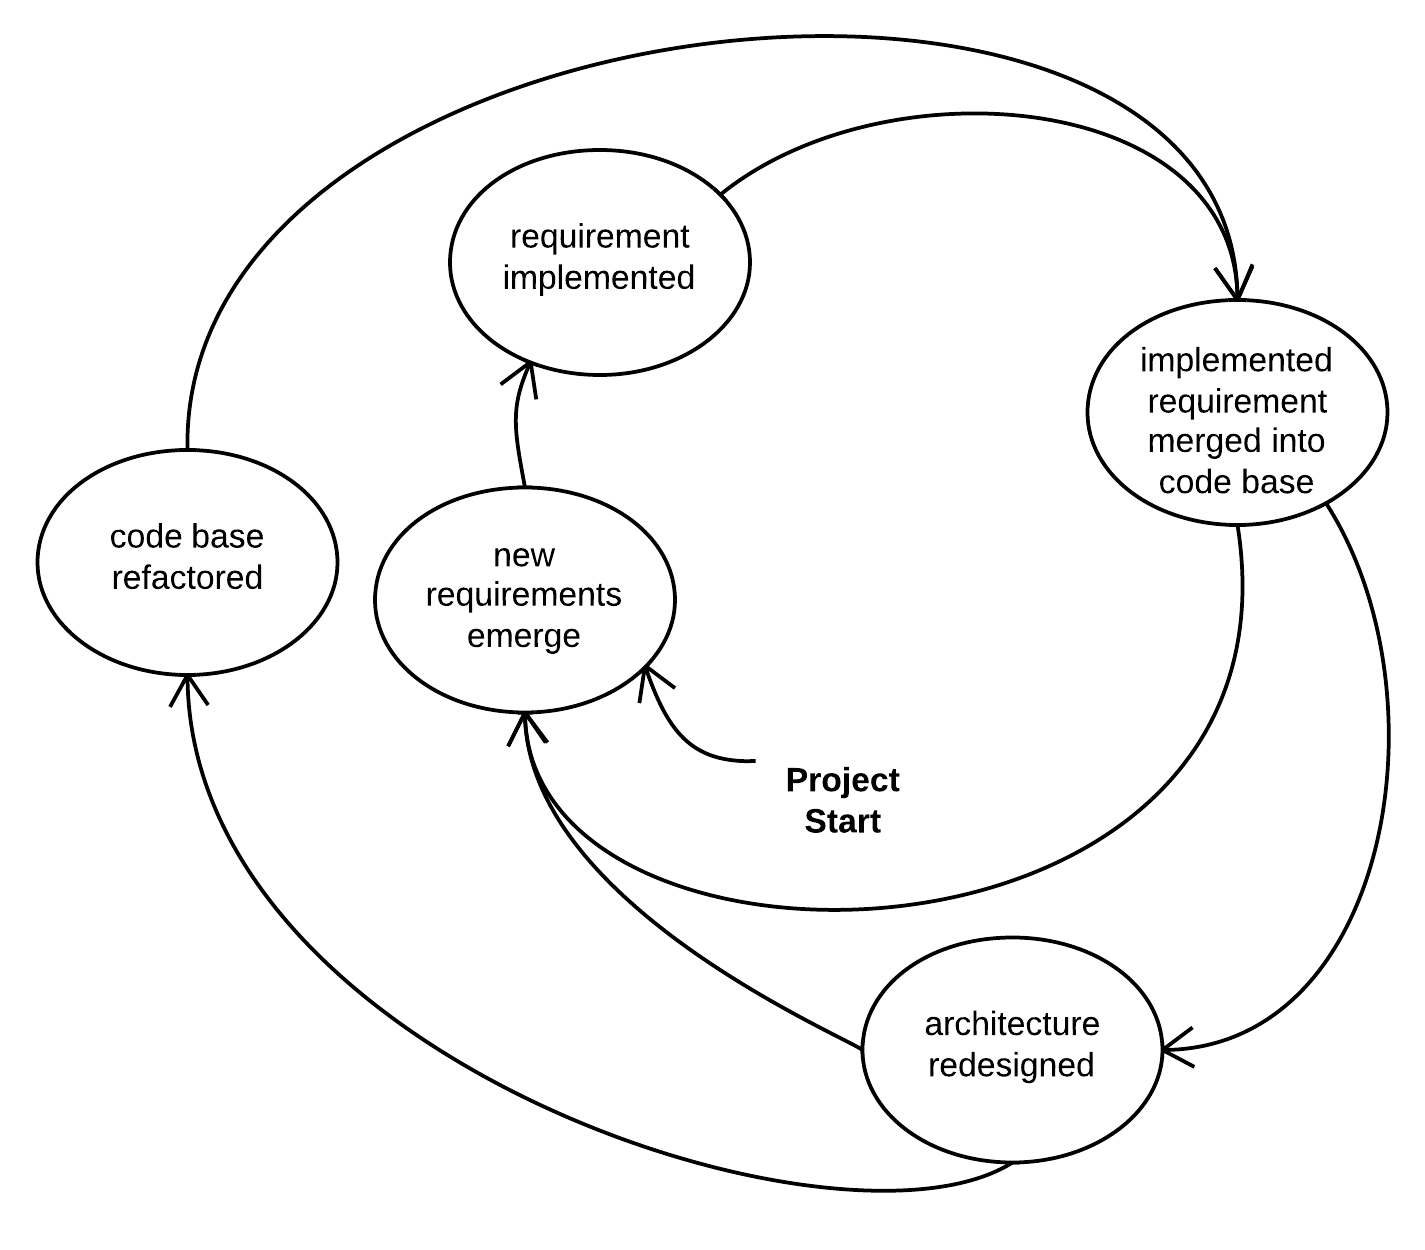
\includegraphics[width=4in]{image/evaluation-development-cycle.png}
\centering
\caption[Development Cycle]{The development cycle that emerged naturally from the individual developers workflow.}
\label{figure:development-cycle}
\end{figure}

\subsection*{Good}
The approach taken was very much a learn as you go-approach. Building an architecture as a first step in the design process can be a good choice. This approach is easier if the architects have extensive knowledge of the systems involved. As this was not the case, the approach allowed the developers to build their knowledge of the existing systems and gems as they went along. Once a knowledge base was reached, a more informed basic architecture could be created.

Doing some implementation early on also reduced the number of pointless goals. If a goal or requirement is created without knowledge of the systems involved, it is likely that the goal will not be reached or that it takes the design in a direction that does not solve other larger goals and requirements.

\subsection*{Bad}
The project went through some major refactoring during development when the architecture was first designed. This was a difficult and time consuming task. An improvement could be made in doing this sooner, but not too soon.

Implementing the requirements outside of the code base made integration more difficult than if the requirement had been implemented within the code base in the first place.

\section{Result Evaluation}
The two types of testing used in the project were testing the assumptions in the preliminary study and one time testing of code functionality

\subsubsection{Testing of preliminary study}
The testing in the preliminary study was done by browsing Twitter for data and aggregating the results in excel or using the Google chrome developer console.

In section~\ref{sec:pre-stream-api-testing}, the Stream API was tested to show what kind coverage of the movies in the Netflix Prize dataset could be expected to get by running the Stream API to harvest tweets. The test was done by manually exploring Twitter web search. This process is prone to human error. However, since the important results were statistical approximations, this type of error can be ignored. The results showed that getting coverage for the entire Netflix data set would take years. The sample size is relatively small and the results could have been better if an automated test was employed. However, the test served primarily as a loose indicator for whether or not the Stream API would serve the purpose as a main channel for harvesting tweets that would cover the dataset. A sample size of 20 assessing 3 different time spans, a month, half a year and a full year seemed sufficient enough for this. The Stream API was thus concluded to not be suitable for the project, but could complement the requirements in the future and was thus implemented, but not focused on.

In section~\ref{sec:pre-twitter-crawl-scrape}, the Crawling and Scraping techniques were tested gradually as they were discovered. The tests used jQuery functions to establish that there was a correspondence between the number of tweets shown on the Twitter search result page and the number of sub elements that were to be extracted from each tweet on the Twitter search result page. The results showed correspondence even as the number of tweets on the page increased gradually. This implied that the technique for selecting the sub elements was most likely correct. This was further confirmed by running the implementation and observing that the tweets that were extracted from the page were actually the same as shown in the browser.

\subsubsection{Testing of code functionality}
The testing of code functionality is described in section~\ref{impl:Testing}. While not as solid as systematic unit and functional testing, the technique verifies at a single point in time that the different parts of the implementation are doing what they should be doing. Though there naturally was more bug fixing, the technique served the needs of the project. The code base ended up being relatively small and thus the amount of manual testing applied was manageable. For a larger project this would not have been feasible as the workload would have increased beyond the point of being manageable

\subsubsection{Types of testing not used}
Testing the predictions with RMSE was one of the main requirements of the project, but was not implemented as predictions could not be made due to the lack of a dataset from Twitter due to constraints and limitations of the Twitter APIs and legal constrains on scraping Twitter.

\section{Issues}\label{sec:issues}

\subsection*{Lack of Twitter dataset}
A dataset that had data from Twitter could not be harvested and built for several reasons.

\subsubsection{API Capability Issues}
The APIs provided by Twitter were not sufficient to harvest data points for the 17770 movies.

The reason was mainly that the Stream API which was the best option for harvesting tweets could only deliver a coverage of 65\% after running for a whole year. If each movie were to be described by 8 or more tweets, the coverage would only be 45\% for this time span. See section~\ref{sec:pre-stream-api-testing}.

The Search API suffered from only delivering tweets within the time span of a single week. There was no explanation of what determined this interval. It was determined that the Search API would not produce better results than the Stream API. See section~\ref{sec:pre-twitter-search}.

The REST API showed promise in harvesting Twitter user relationships, but turned out to be limited to only 15 requests per 15 minute window, or rather one request per minute. If an average of 10 tweets were harvested per movie, it would take 123 days to harvest followers for all tweets harvested. It would take another 123 days to harvest the followees. This further complicated the retrieval of the dataset. See section~\ref{sec:pre-twitter-rest}.

\subsubsection{Legal Issues}
The scraping technique seemed the most promising. It was not formally tested as scraping is not allowed by Twitter and consent from Twitter to employ this technique could not be obtained. See section~\ref{sec:pre-twitter-legal}.

\subsubsection{Consequential Issues}
A major aspect of the project was to use data from Twitter to run predictions on the Netflix Prize Dataset. As a sufficient dataset could not be retrieved from Twitter, these predictions could not be made. The project could consequentially not meet the requirements for doing predictions and testing these predictions with their RMSE.
